\documentclass{article}
\usepackage{tikz}
\usetikzlibrary{shapes.multipart, positioning, arrows.meta}

\begin{document}
\begin{figure}[htbp]
\centering
\vspace{1cm}
\resizebox{\textwidth}{!}{
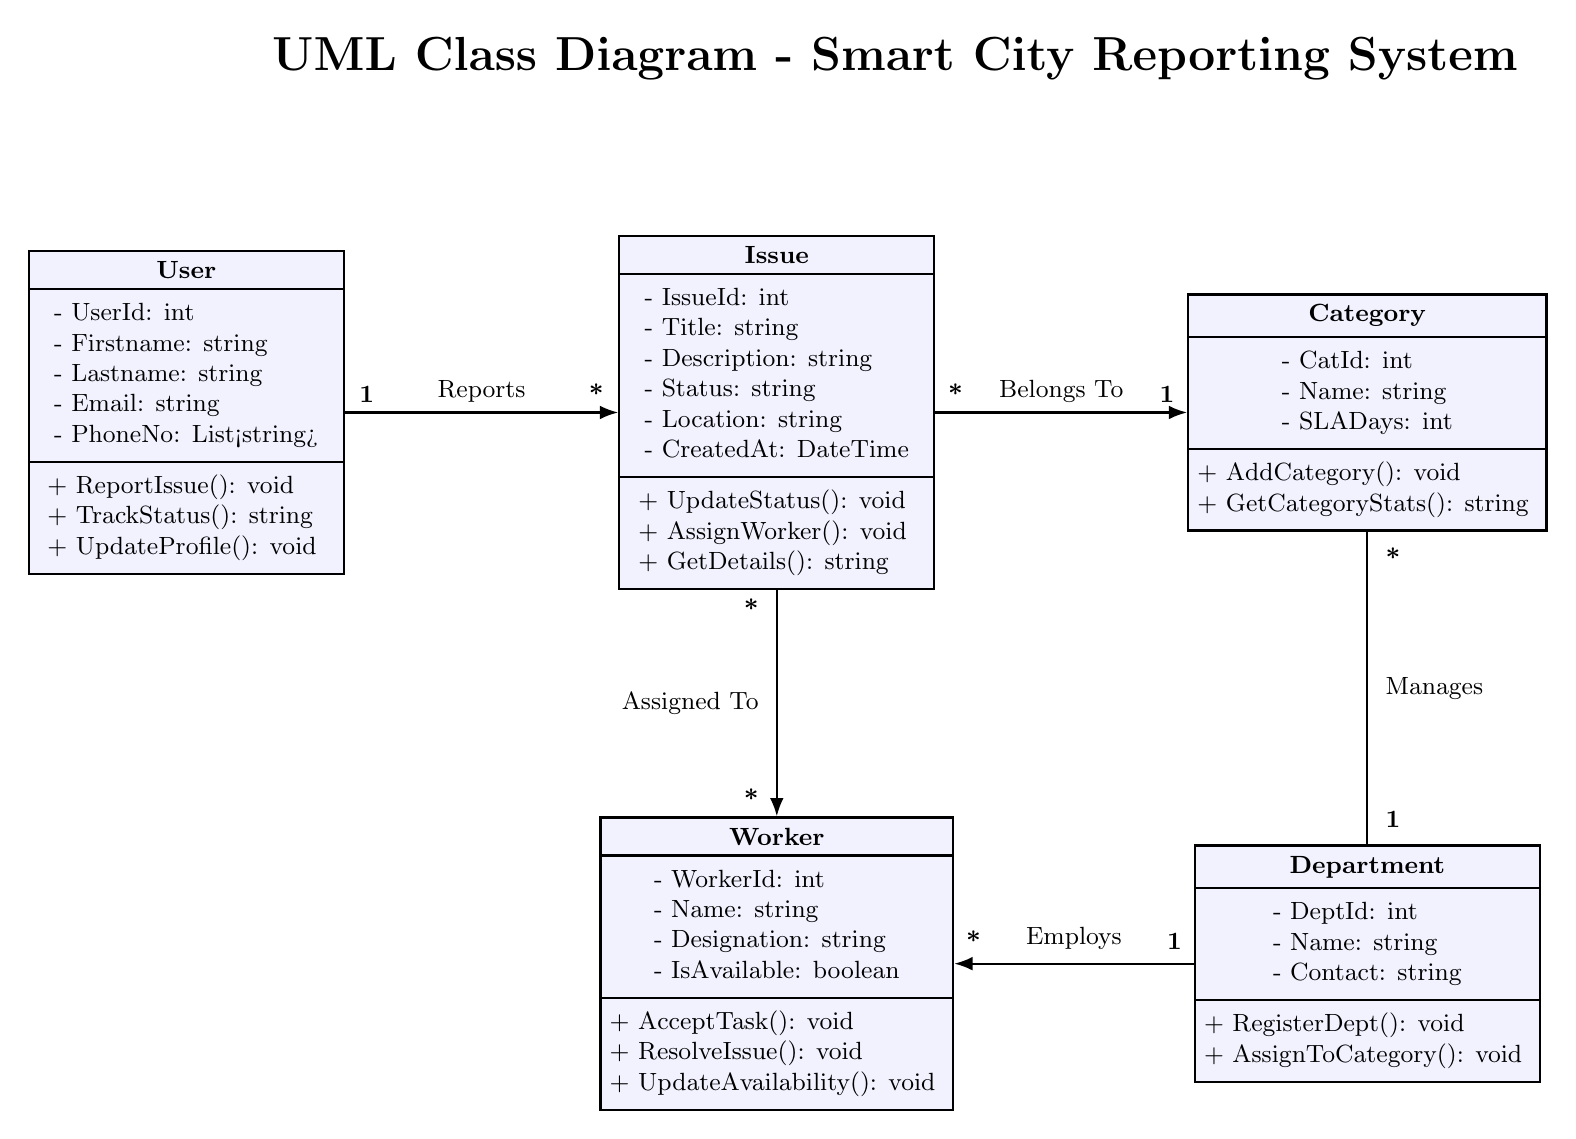
\begin{tikzpicture}[
    >=Latex,
    class/.style={
        draw, rectangle split, rectangle split parts=3,
        minimum width=4cm, align=center, fill=blue!5, thick, font=\small
    }
]

% Title
\node[font=\LARGE\bfseries, align=center] at (1.5, 4.5) {UML Class Diagram - Smart City Reporting System};

% -------------------------
% Class Nodes Definition
% -------------------------

% 1. Issue (Center)
\node[class] (Issue) at (0, 0) {
    \textbf{Issue}
    \nodepart{second}
    \normalfont
    \begin{tabular}{@{}l@{}}
    - IssueId: int \\
    - Title: string \\
    - Description: string \\
    - Status: string \\
    - Location: string \\
    - CreatedAt: DateTime
    \end{tabular}
    \nodepart{third}
    \normalfont
    \begin{tabular}{@{}l@{}}
    + UpdateStatus(): void \\
    + AssignWorker(): void \\
    + GetDetails(): string
    \end{tabular}
};

% 2. User (Left)
\node[class] (User) at (-7.5, 0) {
    \textbf{User}
    \nodepart{second}
    \normalfont
    \begin{tabular}{@{}l@{}}
    - UserId: int \\
    - Firstname: string \\
    - Lastname: string \\
    - Email: string \\
    - PhoneNo: List<string>
    \end{tabular}
    \nodepart{third}
    \normalfont
    \begin{tabular}{@{}l@{}}
    + ReportIssue(): void \\
    + TrackStatus(): string \\
    + UpdateProfile(): void
    \end{tabular}
};

% 3. Category (Right)
\node[class] (Category) at (7.5, 0) {
    \textbf{Category}
    \nodepart{second}
    \normalfont
    \begin{tabular}{@{}l@{}}
    - CatId: int \\
    - Name: string \\
    - SLADays: int
    \end{tabular}
    \nodepart{third}
    \normalfont
    \begin{tabular}{@{}l@{}}
    + AddCategory(): void \\
    + GetCategoryStats(): string
    \end{tabular}
};

% 4. Worker (Bottom Center)
\node[class] (Worker) at (0, -7) {
    \textbf{Worker}
    \nodepart{second}
    \normalfont
    \begin{tabular}{@{}l@{}}
    - WorkerId: int \\
    - Name: string \\
    - Designation: string \\
    - IsAvailable: boolean
    \end{tabular}
    \nodepart{third}
    \normalfont
    \begin{tabular}{@{}l@{}}
    + AcceptTask(): void \\
    + ResolveIssue(): void \\
    + UpdateAvailability(): void
    \end{tabular}
};

% 5. Department (Bottom Right)
\node[class] (Dept) at (7.5, -7) {
    \textbf{Department}
    \nodepart{second}
    \normalfont
    \begin{tabular}{@{}l@{}}
    - DeptId: int \\
    - Name: string \\
    - Contact: string
    \end{tabular}
    \nodepart{third}
    \normalfont
    \begin{tabular}{@{}l@{}}
    + RegisterDept(): void \\
    + AssignToCategory(): void
    \end{tabular}
};

% -------------------------
% Path Connections & Multiplicities
% -------------------------

% User -> Issue
\draw[->, thick] (User.east) -- (Issue.west) 
    node[pos=0.08, above, font=\small\bfseries] {1} 
    node[midway, above, font=\small] {Reports} 
    node[pos=0.92, above, font=\small\bfseries] {*};

% Issue -> Category
\draw[->, thick] (Issue.east) -- (Category.west) 
    node[pos=0.08, above, font=\small\bfseries] {*} 
    node[midway, above, font=\small] {Belongs To} 
    node[pos=0.92, above, font=\small\bfseries] {1};

% Issue -> Worker (Vertical, Assigned To)
\draw[->, thick] (Issue.south) -- (Worker.north) 
    node[pos=0.08, left=0.1cm, font=\small\bfseries] {*} 
    node[midway, left=0.1cm, font=\small] {Assigned To} 
    node[pos=0.92, left=0.1cm, font=\small\bfseries] {*};

% Department -> Worker
\draw[->, thick] (Dept.west) -- (Worker.east) 
    node[pos=0.08, above=0.05cm, font=\small\bfseries] {1} 
    node[midway, above=0.05cm, font=\small] {Employs} 
    node[pos=0.92, above=0.05cm, font=\small\bfseries] {*};

% Department -> Category (No Arrow Head)
\draw[-, thick] (Dept.north) -- (Category.south) 
    node[pos=0.08, right=0.1cm, font=\small\bfseries] {1} 
    node[midway, right=0.1cm, font=\small] {Manages} 
    node[pos=0.92, right=0.1cm, font=\small\bfseries] {*};

\end{tikzpicture}
}
\end{figure}
\end{document}
